%\ctparttext{\color{black}\begin{center}
%		Esta es una descripción de la parte de informática.
%\end{center}}

%\part{Parte de informática}
\chapter{Desarrollo del software: Análisis y diseño}

\section{Objetivos y análisis de requisitos}

Los objetivos que se persiguen al realizar este proyecto son realizar un estudio de distintos modelos de epidemiología. Se pretende comprender cómo afectan sus parámetros y condiciones iniciales a la evolución en el tiempo de estos modelos desde un punto de vista tanto teórico como práctico, apoyándonos en distintas gráficas interactivas para ilustrar dichos comportamientos. Asimismo, se va a analizar la bondad de ajustes de parámetros de algunos de los modelos presentados aplicados a datos reales comprobando cuáles proporcionan mejores resultados en cada caso. Con el fin de satisfacer todos estos objetivos, se ha extraído la siguiente lista de requisitos:

\begin{itemize}
\item \textbf{Requisitos funcionales}
	\begin{itemize}
	\item \textbf{RF1}: Se debe poder modificar los parámetros de las gráficas de los distintos modelos.
	\item \textbf{RF2}: El usuario debe poder elegir con qué modelo quiere trabajar.
	\item \textbf{RF3}: El sistema debe permitir descargar las imágenes de las gráficas obtenidas.
	\item \textbf{RF4}: El sistema debe poder cargar y leer ficheros de datos.
	\item \textbf{RF5}: Se debe visualizar el ajuste obtenido mediante gráficas.
	\item \textbf{RF6}: Para cada ajuste realizado se obtendrá los valores estimados de los parámetros y los errores.
	\item \textbf{RF7}: El sistema debe ser capaz de seleccionar qué modelo se ajusta mejor a los datos. 
	\end{itemize}
\item \textbf{Requisitos no funcionales}
	\begin{itemize}
	\item \textbf{RNF1}: No se podrán ajustar datos de más de un fichero a la vez.
	\item \textbf{RNF2}: Las gráficas deben actualizarse en tiempo real.
	\item \textbf{RNF3}: Se mostrará información de ayuda, en caso de ser necesaria.
	\item \textbf{RNF4}: Se debe poder usar desde el navegador.
	\end{itemize}
\item \textbf{Requisitos de información}
	\begin{itemize}
	\item \textbf{RI1}: Los ficheros de datos con los que se va a trabajar deben ser formato csv con una estructura específica, dependiente de cada modelo.
	\end{itemize}
\end{itemize}

\section{Desarrollo del proyecto}

Actualmente hay diversas metodologías de desarrollo del software. Cada uno de estos modelos consta de una serie de etapas en las que se ha dividido el desarrollo. Para este proyecto, se ha optado por el modelo en espiral. En este modelo el software se desarrolla de forma incremental, es decir, se van añadiendo funcionalidades y mejoras al software según se van evaluando las que ya tiene. Cada bucle o iteración representa un conjunto de actividades. Estas actividades no están fijadas a ninguna prioridad, sino que las siguientes se eligen en función del análisis de riesgo, comenzando por el bucle interior, como se describe en la figura \eqref{modelo_espiral}.

\begin{figure}
\begin{center}
\caption{Modelo en espiral.}
\label{modelo_espiral}
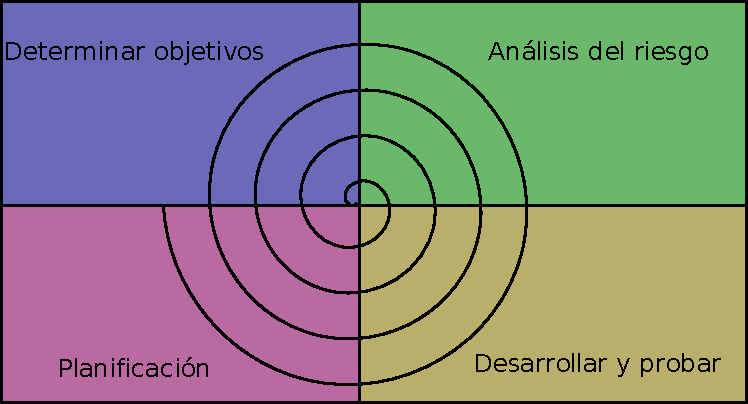
\includegraphics[scale=1]{modelo_espiral}
\end{center}
\end{figure}

Se ha elegido este método de desarrollo ya que se consigue un desarrollo muy estable, pues toda funcionalidad añadida al software es probada y evaluada. De esta forma, aunque el proyecto no esté completo, siempre se tiene una parte funcional, y se va incrementando de forma que siempre disponemos de un producto mínimamente viable. 

\section{Gestión de recursos}

Los proyectos que se pueden realizar dependen en gran medida de los recursos que se pueden destinar a ellos. Se requieren unos elementos mínimos que son indispensables para poder llevarlo a cabo. Por ello, es muy importante contar con los recursos necesarios y gestionarlos de manera adecuada.

\subsection{Recursos humanos}

El proyecto consta de un equipo de 3 personas para llevarlo a cabo:

\begin{itemize}
\item Ana Buendía Ruiz-Azuaga, se encarga de:
	\begin{itemize}
	\item Planificación y análisis del proyecto.
	\item Búsqueda de bibliografía.
	\item Diseño e implementación del proyecto.
	\item Pruebas para el correcto funcionamiento del proyecto.
	\item Redacción de la documentación del proyecto.
	\end{itemize}
\item Tutores: Manuel Pegalajar Cuéllar y Teresa E. Pérez, encargados de:
	\begin{itemize}
	\item Idea original del proyecto.
	\item Proporcionar bibliografía.
	\item Guiar para la redacción de la memoria y documentación.
	\item Supervisar el desarrollo del proyecto.
	\end{itemize}
\end{itemize}

\subsection{Recursos hardware}

Todo el proyecto se va a desarrollar en un ordenador portátil con todo el software y dependencias necesarias. Las especificaciones del portátil son:

\begin{itemize}
\item \textbf{Modelo}: Acer Aspire E-5 574G.
\item \textbf{CPU}: Intel Core i5-6200U.
\item \textbf{RAM} 8GB RAM DDR3.
\item \textbf{Disco duro}: 1TB.
\item \textbf{Precio}: 600€.
\end{itemize}

\subsection{Recursos software}

El proyecto se ha llevado a cabo usando como sistema operativo Ubuntu 20.04 LTS, y se ha usado como lenguaje principal Python.

El software necesario para el proyecto es el siguiente:

\begin{itemize}
\item \textbf{Flask}. Flask es un microframework web en python. Proporciona funcionalidad básica para, de forma sencilla, crear una aplicación web. Una posible alternativa habría sido Django, pero finalmente se ha optado por Flask debido a su simplicidad, legibilidad y que en este proyecto no se requieren muchas de las funcionalidades que Django ofrece integradas. 
\item \textbf{Dash}. Dash es un framework opensource basado en plotly.js y react.js que permite crear fácilmente aplicaciones basadas en datos. En este proyecto se ha usado principalmente por su capacidad de crear gráficas interactivas en tiempo real. 
\item \textbf{VSCode}. Se ha usado VSCode como editor de texto, ya que proporciona una gran cantidad de plugins para cualquier lenguaje, así como integración con git.
\item \textbf{Draw.io}. Para la realización de diagramas de distintas clases, se ha usado el software de dibujo gratuito Draw.io.
\item \textbf{Docker}. Con el fin de simplificar el lanzamiento y ejecución de la aplicación web desarrollada se ha usado docker para virtualizar el entorno y evitar la necesidad de instalar en cualquier máquina el software necesario para ejecutarla.
\item \textbf{Git}. Se ha empleado Git como controlador de versiones, integrado con Github.
\item \textbf{Texmaker}. Para redactar la memoria, se ha usado el editor de LaTeX Texmaker.
\end{itemize}

Todo el software utilizado ha sido gratuito, por lo que no ha tenido coste alguno.

\subsection{Estimación del coste}

A partir de los recursos previamente listados, se va a realizar una aproximación del coste de la consecución del proyecto, considerando que la duración del mismo es de 9 meses.

Para los recursos humanos, dado que se considera que la alumna ha trabajado aproximadamente 450 horas de acuerdo a los créditos correspondientes asignados al TFG, y el gasto aproximado es 15€/h en calidad de alumna de prácticas, se tiene que el coste es de 6.750,00€.

A los tutores, dada su formación profesional se les supone un coste estimado de 50€/h, y aproximando que se dedican 3 horas semanales para la tutorización del proyecto, se tiene que el coste total tras los 9 meses es de 5.400,00€ por tutor.

Dado que el portátil empleado tiene una vida útil estimada de 5 años, le corresponde un coste de 120,00€ durante la realización del proyecto.

Finalmente, dado que todo el software empleado es gratuito, el coste aproximado del proyecto aparece desglosado en la tabla \eqref{tabla_pres}.

\begin{table}[!h]
\caption{Desglose de presupuesto del proyecto.}
\begin{center}
\begin{tabular}{|c c|} 
 \hline
 \textbf{Recursos humanos} & \textbf{Coste (€)} \\ 
 \hline\hline
 Alumna & 6.750,00 \\
 \hline
 Tutor 1 & 5.400,00 \\
 \hline 
 Tutor 2 & 5.400,00 \\
 \textbf{Suma} & \textbf{17.550,00} \\
 \hline
 \textbf{Recursos hardware} & \textbf{Coste (€)} \\ 
 \hline\hline
 Ordenador portátil & 120,00 \\
 \hline
 \textbf{Suma} & \textbf{120,00} \\
 \hline 
 \textbf{Recursos software} & \textbf{Coste (€)} \\
 \hline
  Flask & 0,00 \\
  \hline
  Dash & 0,00 \\
  \hline 
  VSCode & 0,00 \\
  \hline
  TexMaker & 0,00 \\
  \hline 
  \textbf{Suma} & \textbf{0,00} \\ 
 \hline\hline
 \textbf{Suma total} & \textbf{17.670,00} \\
 \hline\hline
 \textbf{Gastos indirectos (18\%)} & \textbf{3.180,60} \\ 
 \hline\hline
 \textbf{Total} & \textbf{20.850,60} \\ 
 \hline\hline
 \textbf{IVA (21\%)} & \textbf{4.378,63} \\ % es .626 
 \hline\hline
 \textbf{Coste final} & \textbf{25.229,23} \\  % es .226
 \hline\hline

 \hline
\end{tabular}
\label{tabla_pres}
\end{center}
\end{table}

\section{Planificación temporal}

Para la realización del proyecto se han distinguido distintas etapas, y en cada una de ellas se ha implementado y trabajado sobre una funcionalidad concreta, de acuerdo al modelo en espiral. Las distintas partes del proyecto han sido:

\begin{itemize}
\item \textbf{T1. Estudio de bibliografía y estado actual de la epidemiología}. Se han consultado diversos libros, artículos y páginas de interés con el fin de comprender mejor y obtener los recursos necesarios para la realización del proyecto. Además, se ha realizado una selección de los modelos a estudiar y tratar durante el desarrollo del mismo.
\item \textbf{T2. Especificación de requisitos}. En base a la información obtenida del proyecto, en esta etapa se han especificado los requisitos que el software debe cumplir.
\item \textbf{T3. Diseño del sistema}. A partir de los requisitos especificados, se ha diseñado la arquitectura del sistema y cómo será la interfaz con la que van a interactuar los usuarios.
\item \textbf{T4. Marco teórico}. Se han indicado conceptos y modelos, así como estudiado las características de estos con el fin de desarrollar la teoría necesaria para trabajar con modelos epidemiológicos. Asimismo, se ha indicado el contexto en el que la epidemiología es de gran utilidad.
\item \textbf{T5. Implementación de los modelos discretos}. Se ha realizado la implementación de los modelos discretos SI, SIR y SIS, incluyendo gráficas interactivas de los mismos.
\item \textbf{T6. Implementación de los modelos continuos}. Se ha realizado la implementación de los modelos continuos SI, SIR y SIS, incluyendo gráficas interactivas de los mismos, al igual que información teórica.
\item \textbf{T7. Ajuste de datos a diversos modelos}. Se ha implementado una funcionalidad para realizar un ajuste de parámetros de acuerdo a un modelo a elegir, o el sistema puede determinar cuál es el modelo que minimiza el error para unos datos dados.
\item \textbf{T8. Documentación del proyecto}. Se ha llevado a cabo la documentación del proyecto durante todo su desarrollo.
\end{itemize}

Con el fin de ayudar a hacer más fácil la comprensión de cómo se ha distribuido el tiempo del proyecto, se ha realizado el diagrama \eqref{fig: planificacion} en el que se puede ver cuánto tiempo se ha dedicado a cada etapa del desarrollo del proyecto durante los 10 meses de duración del mismo.

\begin{figure}[!h]
\begin{center}
\caption{Planificación temporal de las etapas del proyecto.}
\label{fig: planificacion}
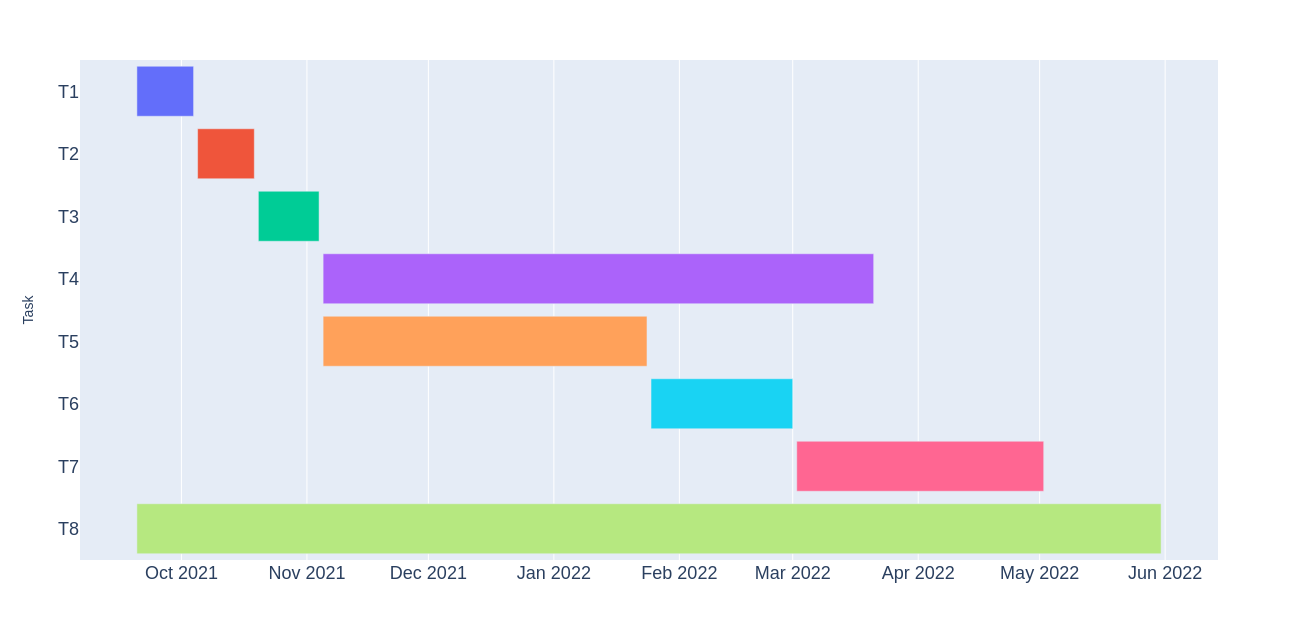
\includegraphics[scale=0.35]{planificacion}
\end{center}
\end{figure}


\section{Diagrama conceptual}

Para el modelado conceptual de la aplicación web, se ha optado por utilizar OOWS (Object-Oriented approach for Web Solutions modelling), que usa modelado de objetos UML y modelos de navegación y presentación usando UML. Así, se expresan las características navegacionales de la aplicación web a la vez que se integra con las restantes vistas del esquema conceptual mediante una notación UML adaptada.

En \eqref{diag: modelo_concep}, se muestra el diagrama conceptual, construido mediante una estrategia top-down:

\begin{figure}[!h]
\begin{center}
\caption{Modelo conceptual de la aplicación web.}
\label{diag: modelo_concep}
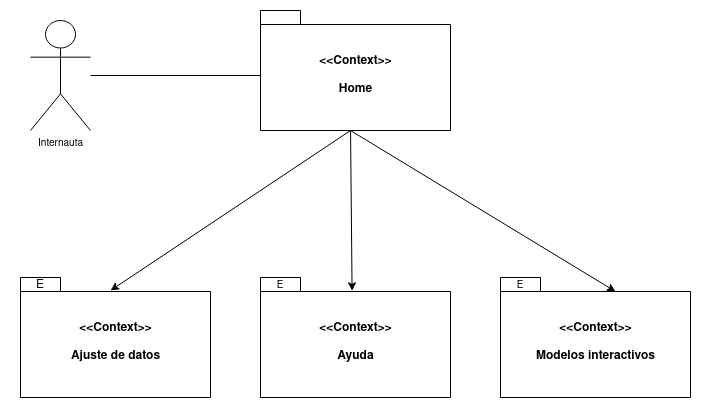
\includegraphics[scale=0.5]{modelo_conceptual-vista-paquetes.drawio}
\end{center}
\end{figure}

En \eqref{diag: modelo_concep_home} se muestra el detalle del contexto de \verb|Home|, en \eqref{diag: modelo_concep_modelos} se ve el detalle de \verb|Modelos Interactivos|, así como en \eqref{diag: modelo_concep_ayuda} el de \verb|Ayuda| y en \eqref{diag: modelo_concep_ajuste} el de \verb|Ajuste de datos|.

\begin{figure}[!h]
\begin{center}
\caption{Modelo conceptual del contexto de Inicio.}
\label{diag: modelo_concep_home}
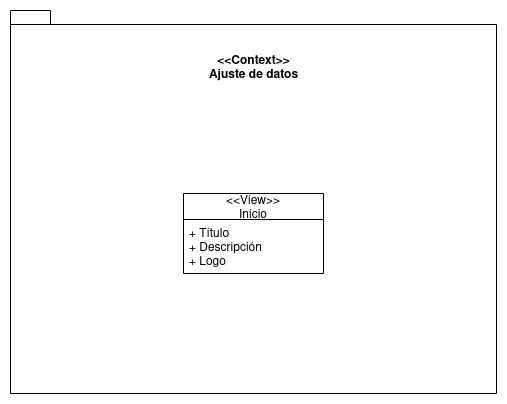
\includegraphics[scale=0.5]{modelo_conceptual-home.drawio}
\end{center}
\end{figure}

\begin{figure}[!h]
\begin{center}
\caption{Modelo conceptual del contexto de Modelos Interactivos.}
\label{diag: modelo_concep_modelos}
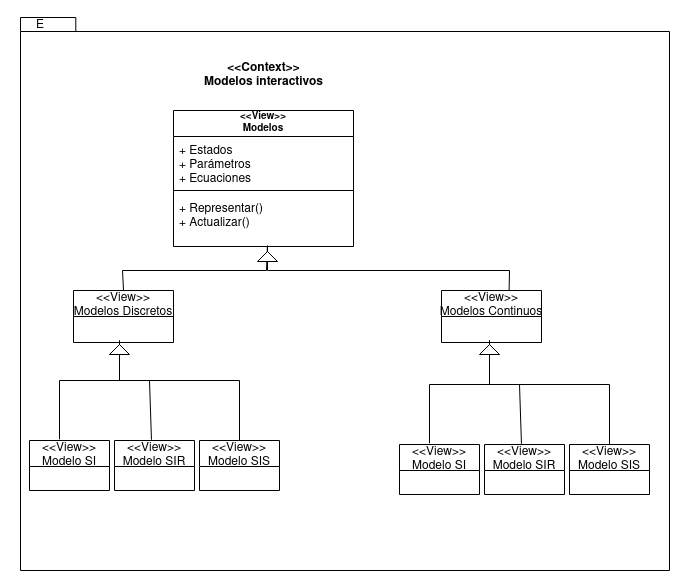
\includegraphics[scale=0.5]{modelo_conceptual-Modelos.drawio}
\end{center}
\end{figure}

\begin{figure}[!h]
\begin{center}
\caption{Modelo conceptual del contexto de Ayuda.}
\label{diag: modelo_concep_ayuda}
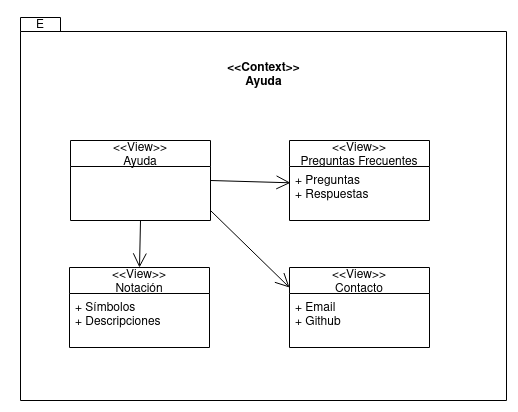
\includegraphics[scale=0.5]{modelo_conceptual-Ayuda.drawio}
\end{center}
\end{figure}

\begin{figure}[!h]
\begin{center}
\caption{Modelo conceptual del contexto de Ajuste de Datos.}
\label{diag: modelo_concep_ajuste}
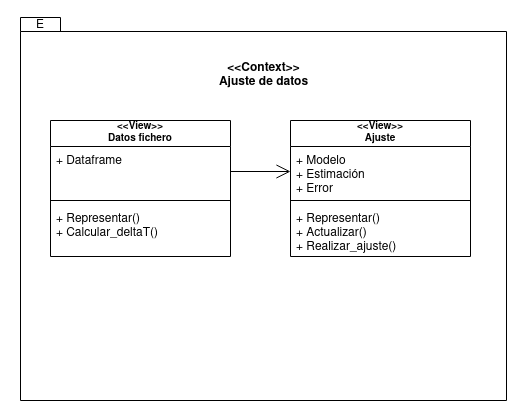
\includegraphics[scale=0.5]{modelo_conceptual-Ajuste.drawio}
\end{center}
\end{figure}





\section{Casos de uso}

A partir de los requisitos listados anteriormente, se obtienen los siguientes casos de uso:

\begin{itemize}
\item \textbf{CU-1}: Modificar parámetro de un modelo.
\item \textbf{CU-2}: Preprocesar entrada.
\item \textbf{CU-3}: Subir fichero de datos.
\item \textbf{CU-4}: Leer fichero de datos.
\item \textbf{CU-5}: Actualizar gráfica.
\item \textbf{CU-6}: Seleccionar modelo de ajuste.
\item \textbf{CU-7}: Realizar ajuste de datos.
\item \textbf{CU-8}: Descargar gráfica.
\end{itemize}

\subsection{Actores del sistema}

\begin{table}[!h]
\begin{tabular}{|c|c|c|c|c|c|c|c|}
\hline
 \rowcolor{azulillo} \textbf{Actor} & \multicolumn{6}{|c|}{Usuario} & {A-1} \\
\hline
 \cellcolor{azulillo} \textbf{Descripción}              & \multicolumn{7}{|c|}{Representa el usuario estándar que va a usar la página web.}           \\
\hline
 \cellcolor{azulillo} \textbf{Características}                 & \multicolumn{7}{|c|}{Interactúa con la aplicación web de forma directa.}             \\
\hline
 \cellcolor{azulillo} \textbf{Relaciones}         & \multicolumn{7}{|c|}{}             \\
\hline
\cellcolor{azulillo} \textbf{Referencias}        & \multicolumn{7}{|c|}{Interviene en los casos de uso CU-1, CU-3 y CU-6.}              \\
\hline
\cellcolor{azulillo} \textbf{Autor}                &   Ana  & \multicolumn{2}{|c|}{\cellcolor{azulillo} \textbf{Fecha}} &  25/04/22   & \multicolumn{2}{|c|}{\cellcolor{azulillo} \textbf{Versión}} & 1.0  \\
\hline
\end{tabular}
\end{table}

\subsection{Diagrama de casos de uso}

Se incluye también el diagrama de los casos de uso, con el fin de ilustrar todos los posibles casos de uso, así como sus relaciones entre ellos. El diagrama resultante puede verse en \eqref{diag: casos_uso}.

\begin{figure}[!h]
\begin{center}
\caption{Diagrama de casos de uso}
\label{diag: casos_uso}
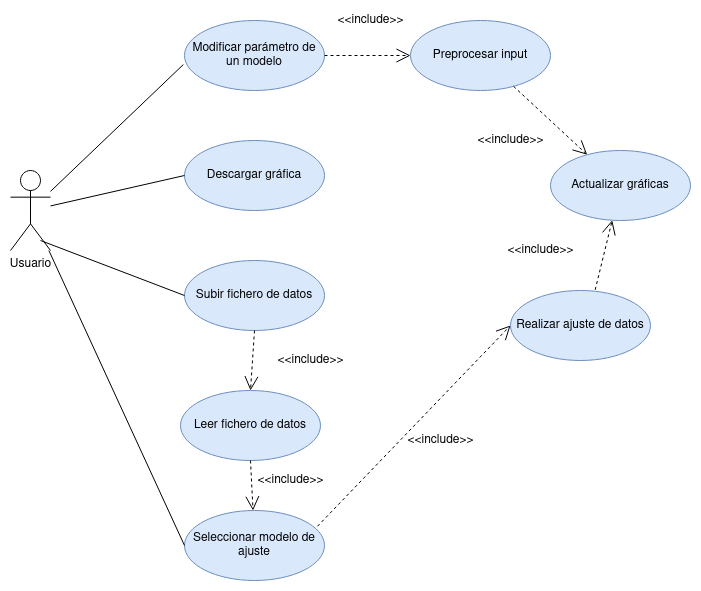
\includegraphics[scale=0.5]{casos_de_uso.drawio}
\end{center}
\end{figure}



\clearpage

\subsection{Plantillas de casos de uso}



\begin{table}[!h]
\begin{tabularx}{\textwidth}{|Y|Y|Y|Y|Y|Y|Y|Y|Y|}
\hline
\rowcolor{azulillo} \multicolumn{2}{|c|}{\textbf{Caso de uso}} & \multicolumn{5}{|c|}{Modificar parámetro de un modelo} & \multicolumn{2}{|c|}{CU-1} \\
\hline
\multicolumn{2}{|c|}{\cellcolor{azulillo} \textbf{Actores}}              & \multicolumn{7}{|c|}{Usuario}           \\
\hline
\multicolumn{2}{|c|}{\cellcolor{azulillo} \textbf{Tipo}}                 & \multicolumn{7}{|c|}{Esencial}             \\
\hline
\multicolumn{2}{|c|}{\cellcolor{azulillo} \textbf{Referencias}}          & \multicolumn{2}{|c|}{RF1}           & \multicolumn{5}{|c|}{CU-2, CU-5}\\
\hline
\multicolumn{2}{|c|}{\cellcolor{azulillo} \textbf{Precondición}}         & \multicolumn{7}{|c|}{Se debe estar trabajando con un modelo.}             \\
\hline
\multicolumn{2}{|c|}{\cellcolor{azulillo} \textbf{Postcondición}}        & \multicolumn{7}{|c|}{Se debe preprocesar la entrada.}              \\
\hline
\multicolumn{2}{|c|}{\cellcolor{azulillo} \textbf{Autor}}               &   Ana  & \multicolumn{2}{|c|}{\cellcolor{azulillo} \textbf{Fecha}} &  25/04/22   & \multicolumn{2}{|c|}{\cellcolor{azulillo} \textbf{Versión}} & 1.0  \\
\hline
\end{tabularx}
\end{table}

\begin{table}[!h]
\begin{tabularx}{\textwidth}{|Y|}
\hline
\cellcolor{azulillo} \textbf{Propósito} \\
\hline
Modificar uno de los parámetros disponibles del modelo para ver cómo afecta al  comportamiento del mismo.   \\
\hline
\end{tabularx}
\end{table}

\begin{table}[!h]
\begin{tabularx}{\textwidth}{|Y|}
\hline
\cellcolor{azulillo} \textbf{Resumen}  \\
\hline
Se modifica uno de los parámetros posibles del modelo, modificando así su comportamiento y visualizando la nueva gráfica resultante.   \\
\hline
\end{tabularx}
\end{table}

\begin{table}[!h]
\begin{tabularx}{\textwidth}{|c|Y|c|Y|}
\hline
\multicolumn{4}{|c|}{ \cellcolor{azulillo}Curso normal} \\
\hline
      1.        &  El usuario modifica un parámetro     &              &              \\
\hline
              &               &       2.       &      Incluir CU-2         \\
\hline
              &               &       3.       &      Incluir CU-5        \\

\hline
\end{tabularx}
\end{table}

\begin{table}[!h]
\begin{tabularx}{\textwidth}{|c|Y|}
\hline
\multicolumn{2}{|c|}{\cellcolor{azulillo} \textbf{Cursos alternos}} \\
\hline
       2a.       &      El formato no es correcto, se asigna un valor por defecto        \\
\hline
       3a.       &      Incluir CU-5        \\
\hline
\end{tabularx}
\end{table}

\begin{table}[!h]
\begin{tabularx}{\textwidth}{|Y|Y|Y|Y|}
\hline
\multicolumn{4}{|c|}{\cellcolor{azulillo} \textbf{Otros datos}} \\
\hline
 \cellcolor{azulillo} \textbf{Frecuencia esperada}             &     Alta          &    \cellcolor{azulillo} \textbf{Rendimiento}          &      Alto        \\
\hline
 \cellcolor{azulillo} \textbf{Importancia}             &      Vital         &     \cellcolor{azulillo} \textbf{Urgencia}         &      Alta        \\
\hline
 \cellcolor{azulillo} \textbf{Estado}             &      Finalizado         &    \cellcolor{azulillo} \textbf{Estabilidad}          &     Alta         \\
\hline
 \cellcolor{azulillo} \textbf{Comentarios}        &  \multicolumn{3}{|c|}{-} \\
\hline
\end{tabularx}
\end{table}





\clearpage

\begin{table}[!h]
\begin{tabularx}{\textwidth}{|Y|Y|Y|Y|Y|Y|Y|Y|Y|}
\hline
\rowcolor{azulillo} \multicolumn{2}{|c|}{\textbf{Caso de uso}} & \multicolumn{5}{|c|}{Preprocesar entrada} & \multicolumn{2}{|c|}{CU-2} \\
\hline
\multicolumn{2}{|c|}{\cellcolor{azulillo} \textbf{Actores} }             & \multicolumn{7}{|c|}{(Sistema)}           \\
\hline
\multicolumn{2}{|c|}{\cellcolor{azulillo} \textbf{Tipo}  }               & \multicolumn{7}{|c|}{Esencial}             \\
\hline
\multicolumn{2}{|c|}{\cellcolor{azulillo} \textbf{Referencias}  }        & \multicolumn{2}{|c|}{RF-1}           & \multicolumn{5}{|c|}{CU-1}\\
\hline
\multicolumn{2}{|c|}{\cellcolor{azulillo} \textbf{Precondición} }        & \multicolumn{7}{|c|}{Se debe haber modificado un parámetro del modelo.}             \\
\hline
\multicolumn{2}{|c|}{\cellcolor{azulillo} \textbf{Postcondición} }       & \multicolumn{7}{|c|}{Se debe actualizar la gráfica. }              \\
\hline
\multicolumn{2}{|c|}{\cellcolor{azulillo} \textbf{Autor}   }             &   Ana   & \multicolumn{2}{|c|}{\cellcolor{azulillo} \textbf{Fecha}} &  25/04/22   & \multicolumn{2}{|c|}{\cellcolor{azulillo} \textbf{Versión}} & 1.0  \\
\hline
\end{tabularx}
\end{table}

\begin{table}[!h]
\begin{tabularx}{\textwidth}{|Y|}
\hline
\cellcolor{azulillo} \textbf{Propósito} \\
\hline
Asegurar el correcto formato y validez del valor introducido. \\
\hline
\end{tabularx}
\end{table}

\begin{table}[!h]
\begin{tabularx}{\textwidth}{|Y|}
\hline
\cellcolor{azulillo} \textbf{Resumen}  \\
\hline
 Se comprueba la validez y formato del valor introducido para asegurar el correcto funcionamiento del modelo.  \\
\hline
\end{tabularx}
\end{table}

\begin{table}[!h]
\begin{tabularx}{\textwidth}{|c|Y|c|Y|}
\hline
\multicolumn{4}{|c|}{\cellcolor{azulillo} \textbf{Curso normal}} \\
\hline
              &               &      1.        &    Se comprueba el tipo de valor (float o entero).         \\
\hline
              &               &      2.        &    Se  comprueba el rango de validez de los valors de cada parámetro.         \\
\hline
              &               &      3.        &    Se comprueba que la población sea constante.          \\
\hline
\end{tabularx}
\end{table}

\begin{table}[!h]
\begin{tabularx}{\textwidth}{|c|Y|}
\hline
\multicolumn{2}{|c|}{\cellcolor{azulillo} \textbf{Cursos alternos}} \\
\hline
        1a       &     Si el valor no es de un tipo válido se sustituye por $0$. \\
\hline
        2b.      &     Si el valor no está en el rango se sustituye por $0$.         \\
\hline

\end{tabularx}
\end{table}

\begin{table}[!h]
\begin{tabularx}{\textwidth}{|Y|Y|Y|Y|}
\hline
\multicolumn{4}{|c|}{\cellcolor{azulillo} \textbf{Otros datos}} \\
\hline
 \cellcolor{azulillo} \textbf{Frecuencia esperada}             &      Alta         &    \cellcolor{azulillo} \textbf{Rendimiento}          &      Alto        \\
\hline
 \cellcolor{azulillo} \textbf{Importancia}             &      Vital         &     \cellcolor{azulillo} \textbf{Urgencia}         &      Alta        \\
\hline
 \cellcolor{azulillo} \textbf{Estado}             &       Finalizado        &    \cellcolor{azulillo} \textbf{Estabilidad}          &    Alta          \\
\hline
 \cellcolor{azulillo} \textbf{Comentarios}        &  \multicolumn{3}{|c|}{-} \\
\hline
\end{tabularx}
\end{table}






\clearpage

\begin{table}[!h]
\begin{tabularx}{\textwidth}{|Y|Y|Y|Y|Y|Y|Y|Y|Y|}
\hline
\rowcolor{azulillo} \multicolumn{2}{|c|}{\textbf{Caso de uso}} & \multicolumn{5}{|c|}{Subir fichero de datos} & \multicolumn{2}{|c|}{CU-3} \\
\hline
\multicolumn{2}{|c|}{\cellcolor{azulillo} \textbf{Actores}}              & \multicolumn{7}{|c|}{Usuario}           \\
\hline
\multicolumn{2}{|c|}{\cellcolor{azulillo} \textbf{Tipo} }                & \multicolumn{7}{|c|}{Esencial}             \\
\hline
\multicolumn{2}{|c|}{\cellcolor{azulillo} \textbf{Referencias}}          & \multicolumn{2}{|c|}{RF4}           & \multicolumn{5}{|c|}{CU-4, CU-5, CU-6, CU-7}\\
\hline
\multicolumn{2}{|c|}{\cellcolor{azulillo} \textbf{Precondición}}         & \multicolumn{7}{|c|}{-}             \\
\hline
\multicolumn{2}{|c|}{\cellcolor{azulillo} \textbf{Postcondición}}        & \multicolumn{7}{|c|}{-}              \\
\hline
\multicolumn{2}{|c|}{\cellcolor{azulillo} \textbf{Autor}  }              &   Ana  & \multicolumn{2}{|c|}{\cellcolor{azulillo} \textbf{Fecha}} &  25/04/22   & \multicolumn{2}{|c|}{\cellcolor{azulillo} \textbf{Versión}} & 1.0  \\
\hline
\end{tabularx}
\end{table}

\begin{table}[!h]
\begin{tabularx}{\textwidth}{|Y|}
\hline
\cellcolor{azulillo} \textbf{Propósito} \\
\hline
El usuario debe poder subir un fichero de datos para trabajar sobre él.  \\
\hline
\end{tabularx}
\end{table}

\begin{table}[!h]
\begin{tabularx}{\textwidth}{|Y|}
\hline
\cellcolor{azulillo} \textbf{Resumen}  \\
\hline
El usuario sube un fichero de datos.    \\
\hline
\end{tabularx}
\end{table}

\begin{table}[!h]
\begin{tabularx}{\textwidth}{|c|Y|c|Y|}
\hline
\multicolumn{4}{|c|}{\cellcolor{azulillo} \textbf{Curso normal}} \\
\hline
      1.        &      El usuario selecciona un fichero de datos.         &              &              \\
\hline
              &               &      2.        &    El sistema sube el fichero de datos seleccionado.          \\
\hline
\end{tabularx}
\end{table}

\begin{table}[!h]
\begin{tabularx}{\textwidth}{|c|Y|}
\hline
\multicolumn{2}{|c|}{\cellcolor{azulillo} \textbf{Cursos alternos}} \\
\hline
      2a.        &    El fichero no tiene formato correcto, por lo que no se deja seleccionarlo.          \\
\hline
\end{tabularx}
\end{table}

\begin{table}[!h]
\begin{tabularx}{\textwidth}{|Y|Y|Y|Y|}
\hline
\multicolumn{4}{|c|}{\cellcolor{azulillo} \textbf{Otros datos}} \\
\hline
 \cellcolor{azulillo} \textbf{Frecuencia esperada}             &     Alta          &    \cellcolor{azulillo} \textbf{Rendimiento}          &      Alto        \\
\hline
 \cellcolor{azulillo} \textbf{Importancia}             &      Vital         &     \cellcolor{azulillo} \textbf{Urgencia}         &      Alta        \\
\hline
 \cellcolor{azulillo} \textbf{Estado}             &      Finalizado         &    \cellcolor{azulillo} \textbf{Estabilidad}          &     Alta         \\
\hline
 \cellcolor{azulillo} \textbf{Comentarios}        &  \multicolumn{3}{|c|}{-} \\
\hline
\end{tabularx}
\end{table}




\clearpage

\begin{table}[!h]
\begin{tabularx}{\textwidth}{|Y|Y|Y|Y|Y|Y|Y|Y|Y|}
\hline
\rowcolor{azulillo} \multicolumn{2}{|c|}{\textbf{Caso de uso}} & \multicolumn{5}{|c|}{Leer fichero de datos} & \multicolumn{2}{|c|}{CU-4} \\
\hline
\multicolumn{2}{|c|}{\cellcolor{azulillo} \textbf{Actores}}              & \multicolumn{7}{|c|}{(Sistema)}           \\
\hline
\multicolumn{2}{|c|}{\cellcolor{azulillo} \textbf{Tipo}}                 & \multicolumn{7}{|c|}{Esencial}             \\
\hline
\multicolumn{2}{|c|}{\cellcolor{azulillo} \textbf{Referencias}}          & \multicolumn{2}{|c|}{RF4}           & \multicolumn{5}{|c|}{CU-3, CU-7}\\
\hline
\multicolumn{2}{|c|}{\cellcolor{azulillo} \textbf{Precondición}}         & \multicolumn{7}{|c|}{Se debe haber subido el fichero a leer.}             \\
\hline
\multicolumn{2}{|c|}{\cellcolor{azulillo} \textbf{Postcondición}}        & \multicolumn{7}{|c|}{Se debe actualizar la gráfica.}              \\
\hline
\multicolumn{2}{|c|}{\cellcolor{azulillo} \textbf{Autor} }               &   Ana   & \multicolumn{2}{|c|}{\cellcolor{azulillo} \textbf{Fecha}} &  25/04/22   & \multicolumn{2}{|c|}{\cellcolor{azulillo} \textbf{Versión}} & 1.0  \\
\hline
\end{tabularx}
\end{table}

\begin{table}[!h]
\begin{tabularx}{\textwidth}{|Y|}
\hline
\cellcolor{azulillo} \textbf{Propósito} \\
\hline
 Leer el fichero para poder trabajar con los datos que contiene.                  \\
\hline
\end{tabularx}
\end{table}

\begin{table}[!h]
\begin{tabularx}{\textwidth}{|Y|}
\hline
\cellcolor{azulillo} \textbf{Resumen}  \\
\hline
 Se lee el fichero de datos cargando estos en memoria.                  \\
\hline
\end{tabularx}
\end{table}

\begin{table}[!h]
\begin{tabularx}{\textwidth}{|c|Y|c|Y|}
\hline
\multicolumn{4}{|c|}{\cellcolor{azulillo} \textbf{Curso normal}} \\
\hline
              &               &      1.        &     Se abre el fichero         \\
\hline
              &               &      2.        &     Se lee el fichero         \\
\hline
\end{tabularx}
\end{table}

\begin{table}[!h]
\begin{tabularx}{\textwidth}{|c|Y|}
\hline
\multicolumn{2}{|c|}{\cellcolor{azulillo} \textbf{Cursos alternos}} \\
\hline
    2a.          &      Si el formato del fichero no es el esperado, se muestra un error.        \\
\hline
\end{tabularx}
\end{table}

\begin{table}[!h]
\begin{tabularx}{\textwidth}{|Y|Y|Y|Y|}
\hline
\multicolumn{4}{|c|}{\cellcolor{azulillo} \textbf{Otros datos}} \\
\hline
 \cellcolor{azulillo} \textbf{Frecuencia esperada}             &      Alta         &    \cellcolor{azulillo} \textbf{Rendimiento}          &      Alto        \\
\hline
 \cellcolor{azulillo} \textbf{Importancia}             &       Vital        &     \cellcolor{azulillo} \textbf{Urgencia}         &      Alta        \\
\hline
 \cellcolor{azulillo} \textbf{Estado}             &       Finalizado        &    \cellcolor{azulillo} \textbf{Estabilidad}          &      Alta        \\
\hline
 \cellcolor{azulillo} \textbf{Comentarios}        &  \multicolumn{3}{|c|}{-} \\
\hline
\end{tabularx}
\end{table}





\clearpage

\begin{table}[!h]
\begin{tabularx}{\textwidth}{|Y|Y|Y|Y|Y|Y|Y|Y|Y|}
\hline
\rowcolor{azulillo} \multicolumn{2}{|c|}{\textbf{Caso de uso}} & \multicolumn{5}{|c|}{Actualizar gráficas} & \multicolumn{2}{|c|}{CU-5} \\
\hline
\multicolumn{2}{|c|}{\cellcolor{azulillo} \textbf{Actores} }             & \multicolumn{7}{|c|}{(Sistema)}           \\
\hline
\multicolumn{2}{|c|}{\cellcolor{azulillo} \textbf{Tipo}  }               & \multicolumn{7}{|c|}{Esencial}             \\
\hline
\multicolumn{2}{|c|}{\cellcolor{azulillo} \textbf{Referencias} }         & \multicolumn{2}{|c|}{RF1, RF2, RF5}           & \multicolumn{5}{|c|}{CU-1, CU-6}\\
\hline
\multicolumn{2}{|c|}{\cellcolor{azulillo} \textbf{Precondición}}         & \multicolumn{7}{|c|}{Se ha modificado un parámetro o ajuste seleccionado.}             \\
\hline
\multicolumn{2}{|c|}{\cellcolor{azulillo} \textbf{Postcondición}  }      & \multicolumn{7}{|c|}{La gráfica se ha actualizado.}              \\
\hline
\multicolumn{2}{|c|}{\cellcolor{azulillo} \textbf{Autor}   }             &   Ana   & \multicolumn{2}{|c|}{\cellcolor{azulillo} \textbf{Fecha}} &  25/04/22   & \multicolumn{2}{|c|}{\cellcolor{azulillo} \textbf{Versión}} & 1.0  \\
\hline
\end{tabularx}
\end{table}

\begin{table}[!h]
\begin{tabularx}{\textwidth}{|Y|}
\hline
\cellcolor{azulillo} \textbf{Propósito} \\
\hline
Actualizar la gráfica para tener la visualización de los datos de acuerdo a las opciones indicadas.   \\
\hline
\end{tabularx}
\end{table}

\begin{table}[!h]
\begin{tabularx}{\textwidth}{|Y|}
\hline
\cellcolor{azulillo} \textbf{Resumen}  \\
\hline
Actualizar la gráfica cuando el usuario realiza una modificación de parámetros o del modelo con el que realizar el ajuste.  \\
\hline
\end{tabularx}
\end{table}

\begin{table}[!h]
\begin{tabularx}{\textwidth}{|c|Y|c|Y|}
\hline
\multicolumn{4}{|c|}{\cellcolor{azulillo} \textbf{Curso normal}} \\
\hline
              &               &      1.        &     Incluir CU-4         \\
\hline
              &               &      2.        &     Representar los datos con el nuevo parámetro.         \\
\hline
\end{tabularx}
\end{table}

\begin{table}[!h]
\begin{tabularx}{\textwidth}{|c|Y|}
\hline
\multicolumn{2}{|c|}{\cellcolor{azulillo} \textbf{Cursos alternos}} \\
\hline
      2a.        &     Si se ha cambiado el modelo con el que realizar el ajuste, incluir CU-7.         \\
\hline
      3a.        &     Representar los datos con el nuevo ajuste.         \\
\hline
\end{tabularx}
\end{table}

\begin{table}[!h]
\begin{tabularx}{\textwidth}{|Y|Y|Y|Y|}
\hline
\multicolumn{4}{|c|}{\cellcolor{azulillo} \textbf{Otros datos}} \\
\hline
 \cellcolor{azulillo} \textbf{Frecuencia esperada}             &     Alta         &    \cellcolor{azulillo} \textbf{Rendimiento}          &      Medio        \\
\hline
 \cellcolor{azulillo} \textbf{Importancia}             &      Vital         &     \cellcolor{azulillo} \textbf{Urgencia}         &     Alta         \\
\hline
 \cellcolor{azulillo} \textbf{Estado}             &       Finalizado        &    \cellcolor{azulillo} \textbf{Estabilidad}          &     Alta         \\
\hline
 \cellcolor{azulillo} \textbf{Comentarios}        &  \multicolumn{3}{|c|}{-} \\
\hline
\end{tabularx}
\end{table}




\clearpage

\begin{table}[!h]
\begin{tabularx}{\textwidth}{|Y|Y|Y|Y|Y|Y|Y|Y|Y|}
\hline
\rowcolor{azulillo} \multicolumn{2}{|c|}{\textbf{Caso de uso}} & \multicolumn{5}{|c|}{Seleccionar modelo de ajuste} & \multicolumn{2}{|c|}{CU-6} \\
\hline
\multicolumn{2}{|c|}{\cellcolor{azulillo} \textbf{Actores}}              & \multicolumn{7}{|c|}{Usuario}           \\
\hline
\multicolumn{2}{|c|}{\cellcolor{azulillo} \textbf{Tipo}}                 & \multicolumn{7}{|c|}{Esencial}             \\
\hline
\multicolumn{2}{|c|}{\cellcolor{azulillo} \textbf{Referencias}}          & \multicolumn{2}{|c|}{RF2}           & \multicolumn{5}{|c|}{CU-5, CU-7}\\
\hline
\multicolumn{2}{|c|}{\cellcolor{azulillo} \textbf{Precondición} }        & \multicolumn{7}{|c|}{Se debe tener leído un fichero de datos.}             \\
\hline
\multicolumn{2}{|c|}{\cellcolor{azulillo} \textbf{Postcondición}}        & \multicolumn{7}{|c|}{Se debe realizar el ajuste con el nuevo modelo elegido.}              \\
\hline
\multicolumn{2}{|c|}{\cellcolor{azulillo} \textbf{Autor}}                &   Ana   & \multicolumn{2}{|c|}{\cellcolor{azulillo} \textbf{Fecha}} &  25/04/22   & \multicolumn{2}{|c|}{\cellcolor{azulillo} \textbf{Versión}} & 1.0  \\
\hline
\end{tabularx}
\end{table}

\begin{table}[!h]
\begin{tabularx}{\textwidth}{|Y|}
\hline
\cellcolor{azulillo} \textbf{Propósito} \\
\hline
Poder elegir el modelo con el que realizar el ajuste de los datos.  \\
\hline
\end{tabularx}
\end{table}

\begin{table}[!h]
\begin{tabularx}{\textwidth}{|Y|}
\hline
\cellcolor{azulillo} \textbf{Resumen}  \\
\hline
Seleccionar el modelo a partir del cuál se va a realizar el ajuste.  \\
\hline
\end{tabularx}
\end{table}

\begin{table}[!h]
\begin{tabularx}{\textwidth}{|c|Y|c|Y|}
\hline
\multicolumn{4}{|c|}{\cellcolor{azulillo} \textbf{Curso normal}} \\
\hline
      1.        &     El usuario selecciona un modelo         &              &              \\
\hline
              &               &      2.        &      Incluir CU-7        \\
\hline
              &               &      3.        &      Incluir CU-5        \\
\hline
\end{tabularx}
\end{table}

\begin{table}[!h]
\begin{tabularx}{\textwidth}{|c|Y|}
\hline
\multicolumn{2}{|c|}{\cellcolor{azulillo} \textbf{Cursos alternos}} \\
\hline
              &       -       \\
\hline
\end{tabularx}
\end{table}

\begin{table}[!h]
\begin{tabularx}{\textwidth}{|Y|Y|Y|Y|}
\hline
\multicolumn{4}{|c|}{\cellcolor{azulillo} \textbf{Otros datos}} \\
\hline
 \cellcolor{azulillo} \textbf{Frecuencia esperada}             &       Alta        &    \cellcolor{azulillo} \textbf{Rendimiento}          &       Alto       \\
\hline
 \cellcolor{azulillo} \textbf{Importancia}             &      Alta         &     \cellcolor{azulillo} \textbf{Urgencia}         &       Alta       \\
\hline
 \cellcolor{azulillo} \textbf{Estado}             &      Finalizado         &    \cellcolor{azulillo} \textbf{Estabilidad}          &      Alta        \\
\hline
 \cellcolor{azulillo} \textbf{Comentarios}        &  \multicolumn{3}{|c|}{-} \\
\hline
\end{tabularx}
\end{table}





\clearpage

\begin{table}[!h]
\begin{tabularx}{\textwidth}{|Y|Y|Y|Y|Y|Y|Y|Y|Y|}
\hline
\rowcolor{azulillo} \multicolumn{2}{|c|}{\textbf{Caso de uso}} & \multicolumn{5}{|c|}{Realizar ajuste de datos} & \multicolumn{2}{|c|}{CU-7} \\
\hline
\multicolumn{2}{|c|}{\cellcolor{azulillo} \textbf{Actores} }             & \multicolumn{7}{|c|}{(Sistema)}           \\
\hline
\multicolumn{2}{|c|}{\cellcolor{azulillo} \textbf{Tipo} }                & \multicolumn{7}{|c|}{Esencial}             \\
\hline
\multicolumn{2}{|c|}{\cellcolor{azulillo} \textbf{Referencias} }         & \multicolumn{2}{|c|}{RF6, RF7}           & \multicolumn{5}{|c|}{CU-3, CU-4, CU-5, CU-6}\\
\hline
\multicolumn{2}{|c|}{\cellcolor{azulillo} \textbf{Precondición}}         & \multicolumn{7}{|c|}{Se debe haber leído un fichero y seleccionado un modelo.}             \\
\hline
\multicolumn{2}{|c|}{\cellcolor{azulillo} \textbf{Postcondición}}        & \multicolumn{7}{|c|}{Actualizar las gráficas}              \\
\hline
\multicolumn{2}{|c|}{\cellcolor{azulillo} \textbf{Autor} }               &   Ana   & \multicolumn{2}{|c|}{\cellcolor{azulillo} \textbf{Fecha}} &  25/04/22   & \multicolumn{2}{|c|}{\cellcolor{azulillo} \textbf{Versión}} & 1.0  \\
\hline
\end{tabularx}
\end{table}

\begin{table}[!h]
\begin{tabularx}{\textwidth}{|Y|}
\hline
\cellcolor{azulillo} \textbf{Propósito} \\
\hline
Obtener una estimación de los parámetros y los errores correspondientes de acuerdo al modelo seleccionado. \\
\hline
\end{tabularx}
\end{table}

\begin{table}[!h]
\begin{tabularx}{\textwidth}{|Y|}
\hline
\cellcolor{azulillo} \textbf{Resumen}  \\
\hline
Se realiza el ajuste de un modelo elegido a los datos leídos. \\
\hline
\end{tabularx}
\end{table}

\begin{table}[!h]
\begin{tabularx}{\textwidth}{|c|Y|c|Y|}
\hline
\multicolumn{4}{|c|}{\cellcolor{azulillo} \textbf{Curso normal}} \\
\hline
     1.         &     Incluir CU-6           &              &              \\
\hline
              &               &    2.          &     Estimar parámetros         \\
\hline
              &               &    3.          &     Calcular errores         \\
\hline
              &               &    4.          &     Incluir CU-5            \\
\hline
\end{tabularx}
\end{table}

\begin{table}[!h]
\begin{tabularx}{\textwidth}{|c|Y|}
\hline
\multicolumn{2}{|c|}{\cellcolor{azulillo} \textbf{Cursos alternos}} \\
\hline
     2a.         &    Si se debe elegir el mejor modelo, se calculan los parámetros para todos los modelos          \\
\hline
     3a.         &    Se calculan los errores para todos los modelos          \\
\hline
     4a.         &    Se elige el mejor modelo de acuerdo a un criterio sobre los errores          \\
\hline
\end{tabularx}
\end{table}

\begin{table}[!h]
\begin{tabularx}{\textwidth}{|Y|Y|Y|Y|}
\hline
\multicolumn{4}{|c|}{\cellcolor{azulillo} \textbf{Otros datos}} \\
\hline
 \cellcolor{azulillo} \textbf{Frecuencia esperada}             &      Alta         &    \cellcolor{azulillo} \textbf{Rendimiento}          &      Alto        \\
\hline
 \cellcolor{azulillo} \textbf{Importancia}             &      Vital         &     \cellcolor{azulillo} \textbf{Urgencia}         &      Alta        \\
\hline
 \cellcolor{azulillo} \textbf{Estado}             &       Finalizado        &    \cellcolor{azulillo} \textbf{Estabilidad}          &     Alta         \\
\hline
\cellcolor{azulillo} \textbf{Comentarios}        &  \multicolumn{3}{|c|}{-} \\
\hline
\end{tabularx}
\end{table}



\clearpage

\begin{table}[!h]
\begin{tabularx}{\textwidth}{|Y|Y|Y|Y|Y|Y|Y|Y|Y|}
\hline
\rowcolor{azulillo} \multicolumn{2}{|c|}{\textbf{Caso de uso}} & \multicolumn{5}{|c|}{Descargar gráfica} & \multicolumn{2}{|c|}{CU-8} \\
\hline
\multicolumn{2}{|c|}{\cellcolor{azulillo} \textbf{Actores} }             & \multicolumn{7}{|c|}{Usuario}           \\
\hline
\multicolumn{2}{|c|}{\cellcolor{azulillo} \textbf{Tipo}}                 & \multicolumn{7}{|c|}{Secundario}             \\
\hline
\multicolumn{2}{|c|}{\cellcolor{azulillo} \textbf{Referencias}}          & \multicolumn{2}{|c|}{RF3}           & \multicolumn{5}{|c|}{}\\
\hline
\multicolumn{2}{|c|}{\cellcolor{azulillo} \textbf{Precondición} }        & \multicolumn{7}{|c|}{-}             \\
\hline
\multicolumn{2}{|c|}{\cellcolor{azulillo} \textbf{Postcondición}}        & \multicolumn{7}{|c|}{-}              \\
\hline
\multicolumn{2}{|c|}{\cellcolor{azulillo} \textbf{Autor} }               &   Ana   & \multicolumn{2}{|c|}{\cellcolor{azulillo} \textbf{Fecha}} &  25/04/22   & \multicolumn{2}{|c|}{\cellcolor{azulillo} \textbf{Versión}} & 1.0  \\
\hline
\end{tabularx}
\end{table}

\begin{table}[!h]
\begin{tabularx}{\textwidth}{|Y|}
\hline
\cellcolor{azulillo} \textbf{Propósito} \\
\hline
Descargar una gráfica generada por la aplicación web. \\
\hline
\end{tabularx}
\end{table}

\begin{table}[!h]
\begin{tabularx}{\textwidth}{|Y|}
\hline
\cellcolor{azulillo} \textbf{Resumen}  \\
\hline
Se descarga la imagen de una gráfica generada. \\
\hline
\end{tabularx}
\end{table}

\begin{table}[!h]
\begin{tabularx}{\textwidth}{|c|Y|c|Y|}
\hline
\multicolumn{4}{|c|}{\cellcolor{azulillo} \textbf{Curso normal}} \\
\hline
     1.         &     Pulsa en descargar imagen           &              &              \\
\hline
              &               &    2.          &     Muestra el selector de archivos         \\
\hline
     3.         &     Selecciona dónde guardar el archivo          &              &             \\
\hline
               &                                            &    4.   & Se genera y descarga la imagen \\
\hline
\end{tabularx}
\end{table}

\begin{table}[!h]
\begin{tabularx}{\textwidth}{|c|Y|}
\hline
\multicolumn{2}{|c|}{\cellcolor{azulillo} \textbf{Cursos alternos}} \\
\hline
     3a.         &    El usuario cancela la descarga.    \\
\hline
\end{tabularx}
\end{table}

\begin{table}[!h]
\begin{tabularx}{\textwidth}{|Y|Y|Y|Y|}
\hline
\multicolumn{4}{|c|}{\cellcolor{azulillo} \textbf{Otros datos}} \\
\hline
 \cellcolor{azulillo} \textbf{Frecuencia esperada}             &      Baja         &    \cellcolor{azulillo} \textbf{Rendimiento}          &      Alto        \\
\hline
 \cellcolor{azulillo} \textbf{Importancia}             &      Baja         &     \cellcolor{azulillo} \textbf{Urgencia}         &      Baja        \\
\hline
 \cellcolor{azulillo} \textbf{Estado}             &       Finalizado        &    \cellcolor{azulillo} \textbf{Estabilidad}          &     Alta         \\
\hline
\cellcolor{azulillo} \textbf{Comentarios}        &  \multicolumn{3}{|c|}{-} \\
\hline
\end{tabularx}
\end{table}

\clearpage

\section{Diagramas de actividad}

Para facilitar la comprensión del funcionamiento de las distintas funcionalidades del sistema, se han realizado diagramas de actividad de sus funcionalidades más importantes, siendo estas la posible modificación de los parámetros de los modelos interactivos y el ajuste de datos subidos mediante un fichero de datos.

El diagrama de actividad correspondiente a la modificación de parámetros en los modelos se muestra en \eqref{diag: actividad_modificacion} y el del ajuste de parámetros se puede ver en \eqref{diag: actividad_ajuste}.

\begin{figure}[!h]
\begin{center}
\caption{Diagrama de actividad de la modificación de parámetros en un modelo.}
\label{diag: actividad_modificacion}
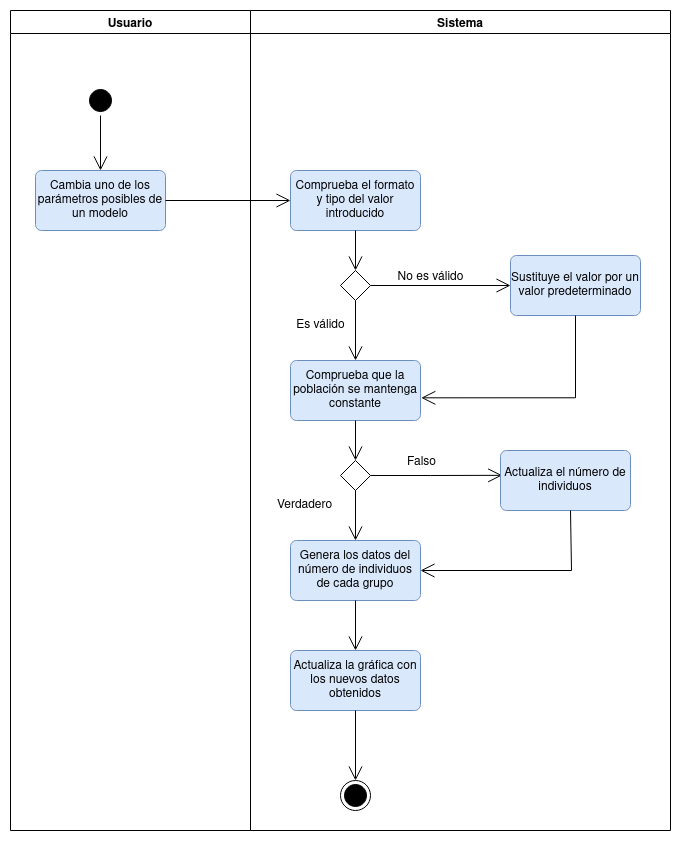
\includegraphics[scale=0.5]{diagrama_actividad-Modificar_parametro.drawio}
\end{center}
\end{figure}

\begin{figure}[!h]
\begin{center}
\caption{Diagrama de actividad del ajuste de datos.}
\label{diag: actividad_ajuste}
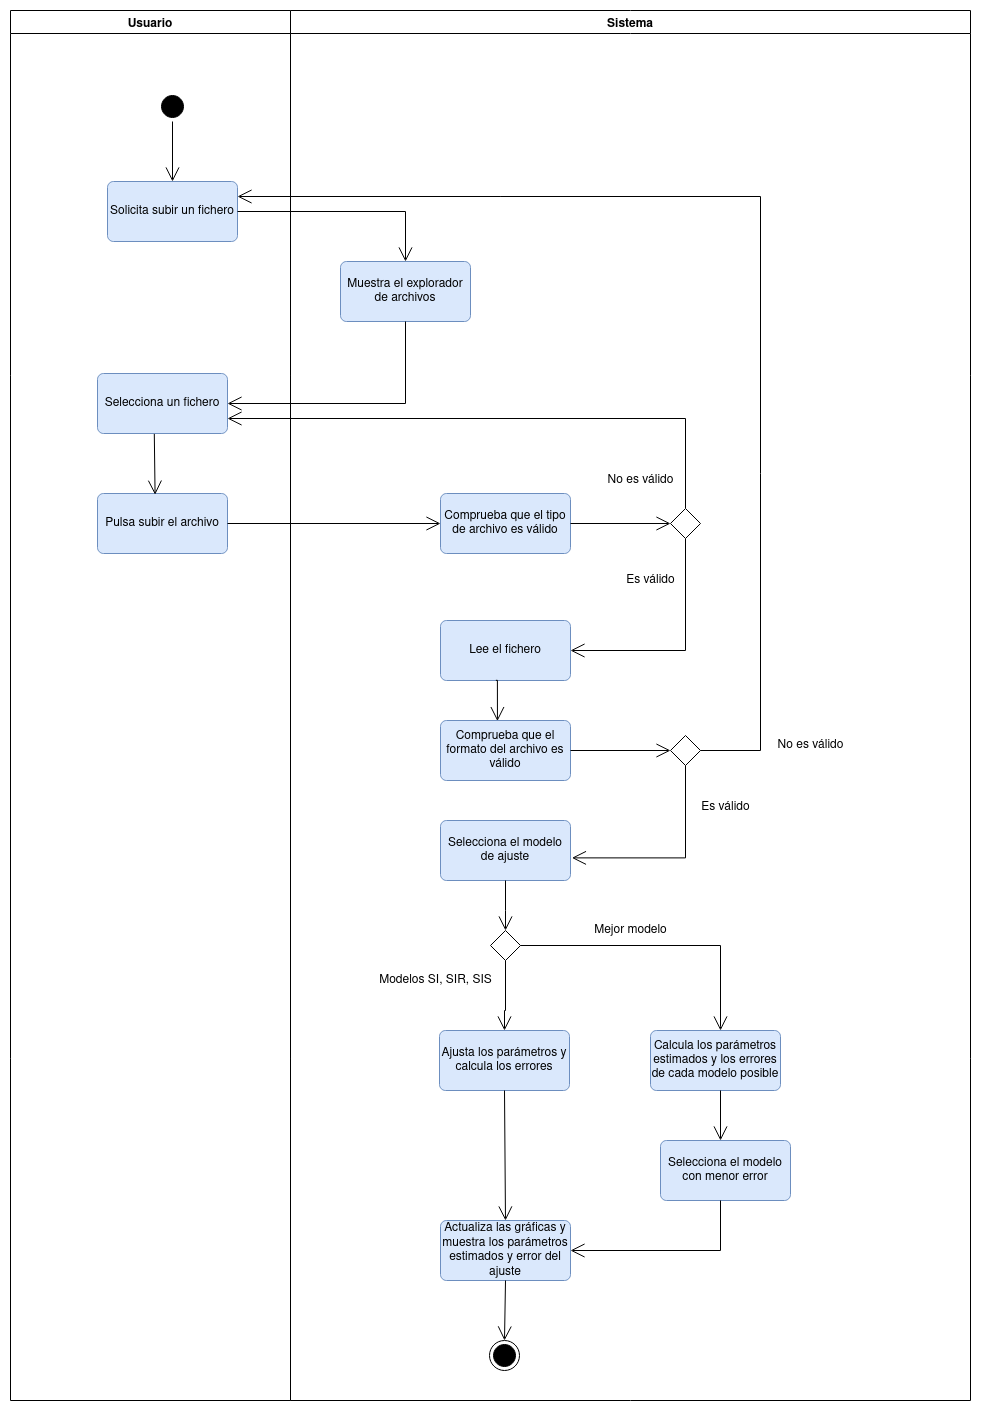
\includegraphics[scale=0.45]{diagrama_actividad-Ajuste_parametros.drawio}
\end{center}
\end{figure}


\section{Pruebas}

A medida que se desarrollaba el proyecto, se han llevado a cabo diversas pruebas de las distintas funcionalidades que se han desarrollado incrementalmente, con el fin de garantizar en todo momento que se disponía de un producto mínimamente viable.

Se han llevado a cabo dos tipos de pruebas:

\begin{itemize}
\item \textbf{Pruebas unitarias:} Tienen como objetivo asegurar el correcto funcionamiento de las funciones creadas de forma independiente de las demás. 
\item \textbf{Pruebas de usuario:} Tratan de simular la interacción entre un usuario y la interfaz del proyecto.
\end{itemize}

\subsection{Pruebas unitarias}

\begin{itemize}
\item \textbf{Preprocesamiento de valores de parámetros.} Se ha probado a introducir diversos valores para los parámetros modificables en los modelos interactivos, con el fin de asegurarnos de que se preprocesan adecuadamente. El comportamiento esperado es sustituir el valor introducido por $0$ en caso de que este sea un carácter o un valor negativo.
\item \textbf{Correcta generación de datos para diversos modelos.} Se han representado gráficamente los datos generados por las funciones de los modelos y contrastando el comportamiento de los datos obtenidos con el descrito en la teoría, asegurando así la correcta generación de los datos de acuerdo a los diversos modelos.
\item \textbf{Subida de ficheros.} Se ha probado a subir ficheros con extensiones permitidas (csv y txt) y comprobado que se han copiado al directorio pertinente para disponer de los ficheros cuando se requiera, así como a subir ficheros con extensiones no permitidas, verificando que se muestra el error pertinente al no permitirse.
\end{itemize}

\subsection{Pruebas de usuario}

\begin{itemize}
\item \textbf{Prueba de población constante.} Si el usuario introduce valores para las condiciones iniciales ($S_0, I_0$ y $R_0$ si es pertinente) tal que su suma no sea $N$ se actualiza el valor de la población de forma que $S_0+I_0+R_0=N$.
\item \textbf{Formato de los valores para parámetros.} Si el usuario introduce un valor de un parámetro con formato incorrecto se sustituye por $0$.
\item \textbf{Condiciones iniciales son números enteros.} Si el usuario introduce un valor no entero positivo se toma como valor real la parte entera del valor introducido por el usuario.
\item \textbf{Subida de fichero inexistente.} Si se trata de subir un fichero al que no se puede acceder o no selecciona ningún fichero antes de pulsar en subir fichero se muestra el error pertinente.
\item \textbf{Interacción con las gráficas.} Los usuarios pueden hacer zoom, desplazarse y obtener el valor numérico de las representaciones gráficas en cada momento en tiempo real, así como descargar las gráficas generadas.
\end{itemize}

\textcolor{red}{Añadiré alguna capturilla cuando compruebe que el aspecto de la aplicación no va a cambiar más (veáse la semana que viene cuando comprobemos que va todo bien)}

\section{Diseño de la interfaz de usuario}

\textcolor{red}{Completar}

\section{Manual de usuario}

\textcolor{red}{Completar}

\section{Datos reales}

\textcolor{red}{Hacer}



















